\documentclass[twocolumn]{article}
\usepackage{amsmath,algorithmic}

% Create link to web,figures (better)
%\usepackage[dvipdfmx]{graphicx,hyperref}
%\usepackage{hyperref}

% Don't link (failsafe option)
\usepackage[dvipdfmx]{graphicx}
\usepackage{url}

%% \setlength{\oddsidemargin}{-0.4mm} 
%% \setlength{\evensidemargin}{\oddsidemargin}
%% \setlength{\textwidth}{170mm} 
\setlength{\textheight}{50\baselineskip}
\addtolength{\textheight}{\topskip}
\setlength{\voffset}{-0.6in}


\bibliographystyle{alpha}

\title{Orthotope Machine}
\author{Takayuki Muranushi}
\begin{document}
\maketitle
\begin{quote}
  In geometry, an {\em orthotope} (also called a hyperrectangle or a box) is
  the generalization of a rectangle for higher dimensions, formally
  defined as the Cartesian product of intervals.

  ``Orthotope'' means ``multidimensional array'' in this document.
\end{quote}

\section{Introduction}

This document describes the {\em Orthotope Machine}, a virtual machine that
operates on multidimensional arrays. The Orthotope Machine is one of the main
components for Paraiso project. The goal of Paraiso project is to create a
high-level programming language for generating massively parallel, explicit
solver algorithms of partial differential equations. 


From computational viewpoint, explicit solvers of partial differential
equations belongs to the algorithm category called stencil codes. Stencil
codes are algorithms that updates the array, each element accessing the nearby
elements in the same pattern (c.f. Fig.\ref{FigureStencilPseudoCode}). Stencil
codes are commonly used algorithms in fields such as solving partial
differential equations and image processing. Code generations and automated
tuning for stencil codes has been studied e.g. \cite{Datta:EECS-2009-177,
  Datta:2008:SCO:1413370.1413375}.

There are many methods other than stencil codes for solving partial
differential equations. They have different merits. A notable project in
progress is Liszt \cite{Chafi:2010:LVH:1932682.1869527}, an embedded
DSL(domain specific language) in programming language Scala, designed for
generating hydrodynamics solver on unstructured mesh.

\begin{figure}
\begin{verbatim}
double a[NY][NX], b[NY][NX];
for (int t=0; t<max_t; ++t) {
  for (int y=1; y<NY-1; ++y) 
    for (int x=1; x<NX-1; ++x) 
      b[y][x] = a[y][x-1] + a[y][x+1] 
              + a[y-1][x] + a[y+1][x];

  for (int y=1; y<NY-1; ++y) 
    for (int x=1; x<NX-1; ++x) 
      a[y][x] += 0.25 * b[y][x];
}
\end{verbatim}
\caption{An example of stencil code.}\label{FigureStencilPseudoCode}
\end{figure}

Many parallel and distributed programming languages has been implemented using
Haskell \cite{CambridgeJournals:114967}. Data Parallel Haskell
\cite{nested-data-parallelism} and
Nepal\cite{springerlink:10.10073-540-44681-8_76} are implementations of NESL,
a language for operating nested arrays.
Accelerate \cite{Chakravarty:2011:AHA:1926354.1926358} and
Nikola \cite{Mainland:2010:NEC:1863523.1863533} are languages to manipulate arrays on GPUs written in Haskell.

We need new languages for parallel hardwares --- this is a long-standing
idea. Many project sought for them, and some failed. Failures from which we
can learn. High Performance Fortran was a very promising approach to introduce
a high-level parallelism in Fortran but, as James Stone told me in Taiwan, and
as is summarized by the project leader
\cite{Kennedy:2007:RFH:1238844.1238851}, it failed.  DEQSOL
\cite{SAGAWANOBUTOSHI:1989-01-15,Kon'no:1986:AIS:324493.325029} was another
project which had design similar to that of Paraiso. The language was
initially designed for Hitachi vector machines. The extension of DEQSOL for
parallel vector machines has been planned \cite{SagawaNobutoshi:1989-03-15}
but seemingly did not realize.

The unique point of Paraiso compared to those projects is its focus on
computational domains that utilize localized access to multidimensional
arrays.

Multidimensional arrays are different from nested arrays. For example in the
pseudocode Fig.\ref{FigureStencilPseudoCode}, in order to calculate {\tt
  b[y][x]} you need to read from {\tt a[y-1][x]} and {\tt a[y+1][x]}, which
are usually located much farther in the memory compared to {\tt a[y][x-32]} or
{\tt a[y][x+64]}. The code generator must be aware of such locality in
multidimensional space.  For most of the cases, the basic equations to be
solved is symmetric under exchange of the axes (X,Y,Z ...). Still, there are
non-negligible differences between the axes from computational point of view,
especially if the multidimensional arrays are stored in row-major or
column-major order. To utilize the cache and/or vector instructions, we need
to know, or decide upon, the order the array is stored in the memory.

In parallel machines, the array must be decomposed and distributed among
computer nodes. It is important to take care of the continuity in
multidimensional space when making the distribution, so that the
communications cost is lowered. If the data to be communicated is stored
sparsely in the memory, it is a good strategy to gather them manually into a
single buffer and to make a single large communication instead of making lots
of small communications. Due to this gather/scattering cost, not making any
decomposition in one or more directions gives higher performance in some
cases.

The Orthotope Machine is designed to capture and utilize these
characteristics of the multidimensional array computations.

\section{Explicit Solvers of Partial Differential Equations}

To begin with, let me describe what kind of problem I want to solve.

\begin{figure}
  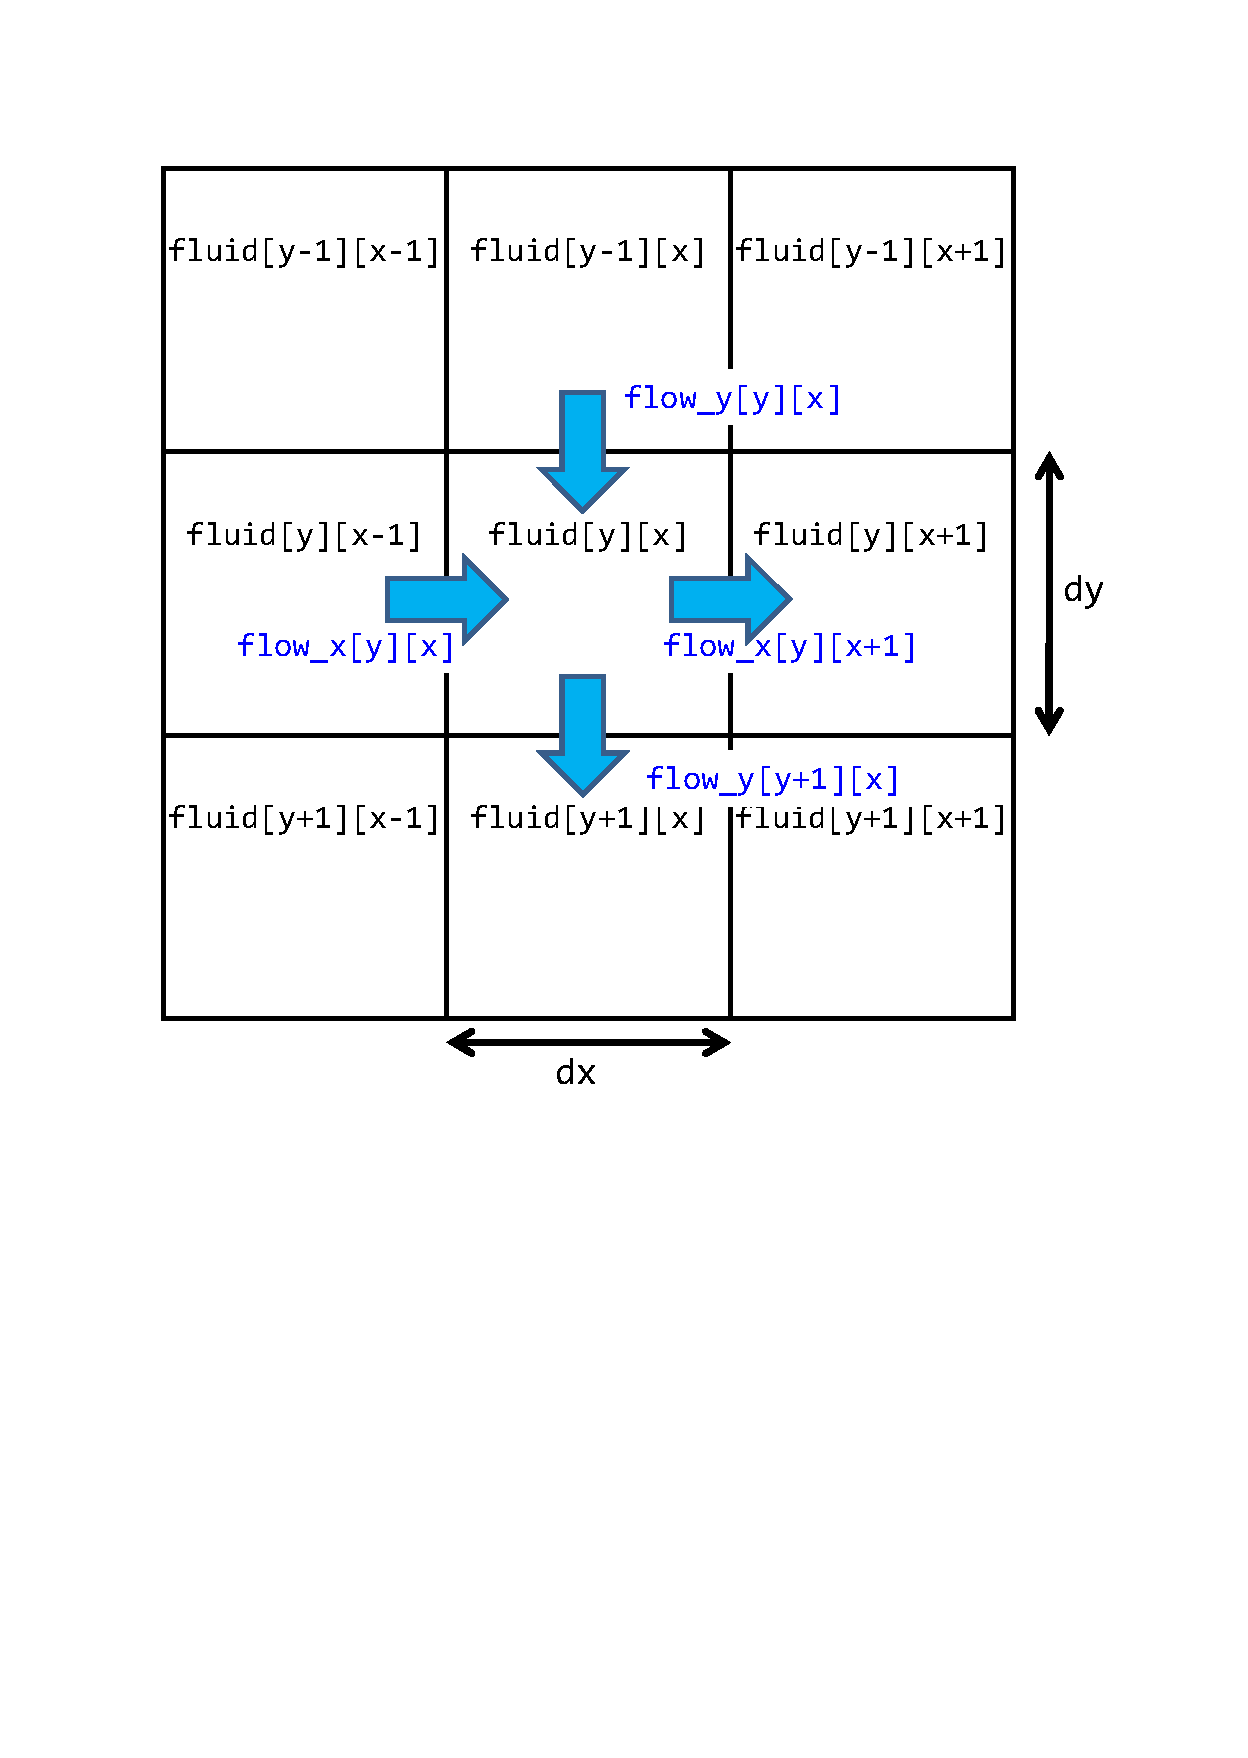
\includegraphics[scale=0.5]{figure/fluid.eps}
  \caption {Schematic image of how a fluid simulator
    works. }\label{FigureFluidScheme}
\end{figure}

\begin{figure*}
\begin{verbatim}
double fluid[NZ][NY][NX];
double flow_x[NZ][NY][NX];
double flow_y[NZ][NY][NX];
double flow_z[NZ][NY][NX];
double dt_local[NZ][NY][NX];

// (1) simulation goes from time t=0 to t=t_max
for (double t=0; t<t_max; t+=dt) {

  // (2) calculate the timescale for each mesh
  for (int z=1; y<NZ-1; ++z) 
    for (int y=1; y<NY-1; ++y) 
      for (int x=1; x<NX-1; ++x) 
        dt_local[z][y][x]=timescale(fluid[z][y][x]);

  // (3) calculate the minimum timescale
  double dt=max_t;
  for (int z=1; y<NZ-1; ++z) 
    for (int y=1; y<NY-1; ++y) 
      for (int x=1; x<NX-1; ++x) 
        dt=min(dt, dt_local[z][y][x]);

  // (4) calculate the flow for each direction
  for (int z=1; y<NZ; ++z) {
    for (int y=1; y<NY; ++y) { 
      for (int x=1; x<NX; ++x) { 
        flow_x[z][y][x]=calc_fx(fluid[z][y][x-1], fluid[z][y][x]);
        flow_y[z][y][x]=calc_fy(fluid[z][y-1][x], fluid[z][y][x]);
        flow_z[z][y][x]=calc_fz(fluid[z-1][y][x], fluid[z][y][x]);
      }
    }
  }

  // (5) move the fluid according to the flow
  for (int z=1; y<NZ-1; ++z) 
    for (int y=1; y<NY-1; ++y) 
      for (int x=1; x<NX-1; ++x)
          fluid[z][y][x] += dt*(
            (flow_x[z][y][x]-flow_x[z][y][x+1])/dx +
            (flow_y[z][y][x]-flow_x[z][y+1][x])/dy +
            (flow_z[z][y][x]-flow_x[z+1][y][x])/dz);

}
\end{verbatim}
  \caption{A pseudocode showing the typical design of a hydrodynamic
    equations solving algorithm.  c.f.  Fig. \ref{FigureFluidScheme}
  }\label{FigureHydroPseudoCode}
\end{figure*}

Let us take for example a hydrodynamics solver that represent the
fluid by a mesh structure c.f. Fig. \ref{FigureFluidScheme}. Each mesh
stores the amount of fluid that is in that mesh. The solver's
algorithm is to calculate the flows of the fluid accross the mesh
boundaries, and add/subtract the amount of fluid.

Fig. \ref{FigureHydroPseudoCode} shows a pseudocode for a
three-dimensional hydrodynamic equations solver. Although it is a bit
simplified to be a real solvers, it shows what components needed to
build one.

A common task for the solver is to simulate the evolution of the fluid for a
certain interval of time, say, $0 < t < t_{\mathrm max}$ (1). In the each step
of the simulation, the time {\tt t} increases by a certain amount {\tt dt}.
In many problems, the time-step {\tt dt} is not a constant but depends on the
state of the fluid. In such case, you need to calculate the time-steps adequate
for the fluid state of every mesh (2), and then perform reduction over the
entire computational domain to calculate the smallest {\tt dt} (3). Then,
amount of fluid flow across X, Y, and Z mesh boundaries are calculated from
the fluid state of the meshes that are adjacent to the boundaries (4). 

To generate a real-world fluid solver, there are more complexity compared to
the example in Fig. \ref{FigureHydroPseudoCode}. First, the {\tt fluid} has
not one but several component. For example, we typically need five 3D arrays
(or an array of a struct with five elements) to solve hydrodynamics. They are
density, three components of the velocity, and energy. For
magneto-hydrodynamics, we need eight components. For general relativity we
need twenty-one.

Second, the size of the stencil (the number of input mesh needed to calculate
the answer for one mesh) is larger. {\tt calc\_fx} in
Fig. \ref{FigureHydroPseudoCode} reads two mesh. In real solvers, they may
read four, six or more meshes, to achieve higher-order interpolation in space.
Third, the entire solver will be replicated several times, to achieve
higher-order time integral. Runge-Kutta method is a well known example of such
a technique. This also make the stencil larger.

Too large stencil is a bad thing. We need to perform duplicated calculations,
and we need communication buffer so large that distributed computation do not
contribute to better performance. So we need to split the algorithm into
several components with smaller stencil. Splitting it into too many pieces, is
again not a good idea. We must search for the middle path.

To get a feeling of a real ``real-world solver,'' please look at {\tt
  proceed} function of my magneto-hydrodynamics solver I'm working
right now :
\url{https://github.com/nushio3/nmhd/blob/master/src/library/mhd_solver.inl}
. I just wanted you to see how dirty the code is and how it repeats
itself. The code is actually generated from a more compact, but less
readable ruby script :
\url{https://github.com/nushio3/nmhd/blob/master/src/library/mhd_solver.inlrb}
.



\section{Overall Design of Paraiso}

\begin{table*}
  \begin{tabular}{|l|l|l|}
    \hline 
    Language                             &  Sample code & Handled by \\
    \hline 
    DPDEL                                & Fig.\ref{FigureDPDEL1},\ref{FigureDPDEL2} & DPDEL monad, quasiquoter and parser     \\
    Primordial Orthotope Machine AST     & Fig.\ref{FigureOMInst} & Orthotope Machine divider \\
    Distributed Orthotope Machine AST    & & Orthotope AST optimizer and compiler \\
    Native codes (Fortran,C,CUDA,OpenCL with MPI) & Fig.\ref{FigureHydroPseudoCode} & Native compilers\\
    Executables                          & & Real machines \\
    \hline
  \end{tabular}
  \caption{
    The software stack of Paraiso, through which DPDEL programs are translated to executables.
  }\label{TableSoftwareStack}
\end{table*}

In this section I briefly describe the overall design of Paraiso, to clarify
the Orthotope Machine's role in it. Please also
c.f. \url{http://paraiso-lang.org/wiki/index.php/Grand_Design}.

Paraiso translates the input programs into native programs with several steps:
c.f. Table \ref{TableSoftwareStack}. The input language is DPDEL (Discretized
Partial Differential Equation Language); the language to describe the
numerical simulation algorithms, in as simple form as possible
c.f. \url{http://paraiso-lang.org/wiki/index.php/DPDEL}.  Then it is
translated to Orthotope Machine (OM) program. Its name used to be Virtual
Vector Machine (VVM) in original Paraiso proposal c.f.
\url{http://paraiso-lang.org/wiki/index.php/VVM}. There are two versions of
Orthotope Machine: one is Primordial OM, the other is Distributed OM.  DPDEL
program is first translated to Primordial OM program, on which it can use
arbitrary large arrays. Then ``machine division'' operations are applied,
according to the hardware specifications, producing Distributed OM
instructions. Distributed OM instructions are then translated to native
codes. Native codes are compiled by existing compilers, and finally, all
programs are executable.



\subsection{Discretized Partial Differential Equation Language (DPDEL)}

DPDEL program is constructed within a monad: This technique is
described in tanakh's blog \url{http://d.hatena.ne.jp/tanakh/20070918}
and is featured in the first prototype of Paraiso. The monad is called
{\tt Dsl} and defined in
\url{https://github.com/nushio3/Paraiso/blob/master/attic/paraiso-2008-ODEsolver/Paraiso.hs}.


Fig.\ref{FigureDPDEL1} shows the possible DPDEL program. Although it is fairly
readable, it has some shabby points.
\begin{itemize}
  \item Calculations for X,Y,Z directions are repeated,
  \item Vectors are represented in scary ways: {\tt ((-1):.0:.0)},
  \item Most part of the program is to assign an expression {\tt expr} to a
    new AST node {\tt a}, but you cannot write {\tt a <- expr} since lhs is
    also an expression and both must have the same type; {\tt expr} cannot be
    a monad that returns {\tt expr}.  Expression must go through some function
    e.g. {\tt bind :: AST a -> DPDEL (AST a)}.
  \item You are forced to use customized operators {\tt+. *.} ... instead of
    usual operators {\tt+ *}... . This may not happen in the arithmetric
    operators, but at least it surely happens for comparison operators such as
    {\tt>}, because their type is {\tt a -> a -> Bool}. You cannot get it have
    the type {\tt AST a -> AST a -> AST Bool}. This barrier is also observed
    in Nikola, a DSL for GPU in Haskell
    \cite{Mainland:2010:NEC:1863523.1863533}.
\end{itemize}

Fig.\ref{FigureDPDEL2} shows another possible version of DPDEL with
above drawbacks removed.  First improvement is the concept of Axis. In
the sample code, axis has two role.  One is to specify a certain
component of three-dimensional vector, e.g. {\tt flow\_axis}. The
other is to shift the indices for three-dimensional arrays. The
indices are represented as lambda-bound variable {\tt o} and shifted
like {\tt [o+axis]}.

This double-roled Axis is invented for my magnetohydrodynamics
program. The two role combined, it really helps writing template
functions, instantiated three times, each of which handles one of
X,Y,Z directions. The concept of Axis is defined in
\url{https://github.com/nushio3/nmhd/blob/master/src/library/direction.h}
as a set of dummy structs {\tt XAxis, YAxis, Zaxis} etc. It is
extensively used to construct three-dimensionally accessible arrays
\url{https://github.com/nushio3/nmhd/blob/master/src/library/crystal.h}
as well as to write the main program.

But how does Haskell know that the name {\tt flow\_axis} is related with the
name {\tt axis}? Isn't {\tt flow\_axis} a single name identifier in Haskell
syntax? Here comes the second point.

We introduce {\bf \tt qb}, quasiquote-and-bind operation. This lifts the
constraints coming from the Haskell syntax. It parses its argument string and
does several things: it changes {\tt flow\_axis} into something like {\tt
  getComponent axis flow}. It renames the arithmetic operators
appropriately. It translates {\tt [o+axis]} into type-correct expression like
{\tt [o+getUnitVector axis]}. It has implicit antiquotes. Finally, {\tt qb}
adds {\tt bind} to the entire expression. {\tt qb} grants us magical power.

Well, things may not go too well with {\tt qb}. We may find some of the
facilities described above impossible to implement. We may need several
quasiquoters instead of just one. Even so, use of quasiquote is essential in
making DPDEL syntax simpler.

\begin{figure*}
\begin{verbatim}
timescale = ...
calcFX f1 f2 = ...
calcFY f1 f2 = ...
calcFZ f1 f2 = ...

proceed :: DPDEL ...
proceed = do
  t <- input $ Orthotope0
  fluid <- input $ Orthotope3
  dtLocal <- bind $ timescale fluid
  dt <- bind $ reduce Min dtLocal

  flowX <- bind $ calcFX fluid (shift ((-1):.0:.0) fluid)
  flowY <- bind $ calcFY fluid (shift (0:.(-1):.0) fluid)
  flowZ <- bind $ calcFZ fluid (shift (0:.0:.(-1)) fluid)
  
  newFluid <- bind $ fluid +. dt *. (
    (flowX -. shift (1:.0:.0) flowX)/.dx +
    (flowY -. shift (0:.1:.0) flowY)/.dy +
    (flowZ -. shift (0:.0:.1) flowZ)/.dz )

  output (t+dt) t
  output newFluid fluid

\end{verbatim}
\caption{A DPDEL monad that corresponds to the pseudocode in
  Fig. \ref{FigureHydroPseudoCode}.}\label{FigureDPDEL1}
\end{figure*}

\begin{figure*}
\begin{verbatim}
timescale = ...
calcF axis f1 f2 = ...

proceed :: DPDEL ...
proceed = do
  t <- input $ Orthotope0
  fluid <- input $ Orthotope3
  dtLocal <- bind $ timescale fluid
  dt <- bind $ reduce Min dtLocal

  flow <- forAxes (\axis ->
    [qb| o -> calcF axis fluid[o] fluid[o-axis]] )

  
  updates <- forAxes (\axis -> [qb| o-> (flow_axis[o] - flow_axis[o+axis]) / dr_axis ]

  newFluid = [qb| o-> fluid[o] + dt * (sum updates)[o]]

  output (t+dt) t
  output newFluid fluid

\end{verbatim}
\caption{A more sophisticated DPDEL code using quasi-quote and Axis. {\bf qb}
  is a quoted bind. The argument of {\bf qb} is parsed by a separate parser
  that understands e.g. the Einstein rules, and a {\bf bind} is added.
  Compare with Fig. \ref{FigureDPDEL1}.}\label{FigureDPDEL2}
\end{figure*}

\subsection{Orthotope Machine}

DPDEL programs are translated into programs for the Orthotope Machine,
the main topic of this document. The OM program describes dataflow
from one orthotope to others, in static single assignment (SSA) style
machine-language-flavor program, forming a directed asyclic graph. The
DPDEL program in Fig. \ref{FigureDPDEL2} will translate to something
like Fig. \ref{FigureOMInst} . Also look at
\url{https://github.com/nushio3/Paraiso/blob/master/attic/paraiso-2010-lifegame/}
for the working example, the second prototype of Paraiso. When you
{\tt make} this program, you'll see the Conway's game of life
running. {\tt Main.hs} contains the program for the cellular
automata. {\tt VVM.hs} defines the instruction set and the syntax
tree, and {\tt VVMCompiler.hs} is a compiler.

\begin{figure*}
\begin{verbatim}
t <- input 
fluid <- input
dtLocal <- ...
dt <- reduce dtLocal

a1 <- shift ((-1):.0:.0) fluid
flowX   <- arith calcFX fluid a1
a2 <- shift (0:.(-1):.0) fluid
flowY   <- arith calcFY fluid a2
a3 <- shift (0:.0:.(-1)) fluid
flowZ   <- arith calcFZ fluid a3

a4 <- shift (1:.0:.0) flowX
a5 <- arith (-) flowX a4
a6 <- arith (/) a5 dx
a7 <- shift (0:.1:.0) flowY
a8 <- arith (-) flowY a7
a9 <- arith (/) a8 dy
a10 <- shift (0:.0:.1) flowZ
a11 <- arith (-) flowZ a10
a12 <- arith (/) a11 dz
a13 <- arith (+) a6 a9
a14 <- arith (+) a13 a12
a15 <- arith (*) a14 dt
a16 <- arith (+) a15 fluid

newT <- arith (+) t dt

output newT t
output a16 fluid
\end{verbatim}
  \caption{A sketch of how an Orthotope Machine instruction will look
    like.}\label{FigureOMInst}
\end{figure*}


\clearpage


\section{Definitions of Orthotope, Orthotree, and Distributed Orthotope}

\section{API for Orthotope Machine}


\section{Hardware Model}

Machine division is performed to fit a target parallel computer, so we
need to describe the hardware configuration in machine-readable form.
Fig.~\ref{FigureHardware} shows a hardware model, and is generated by
graphViz program --- from machine readable {\tt .dot} graph
definition. So there's some hope. 

\begin{figure*}
  \begin{center}
    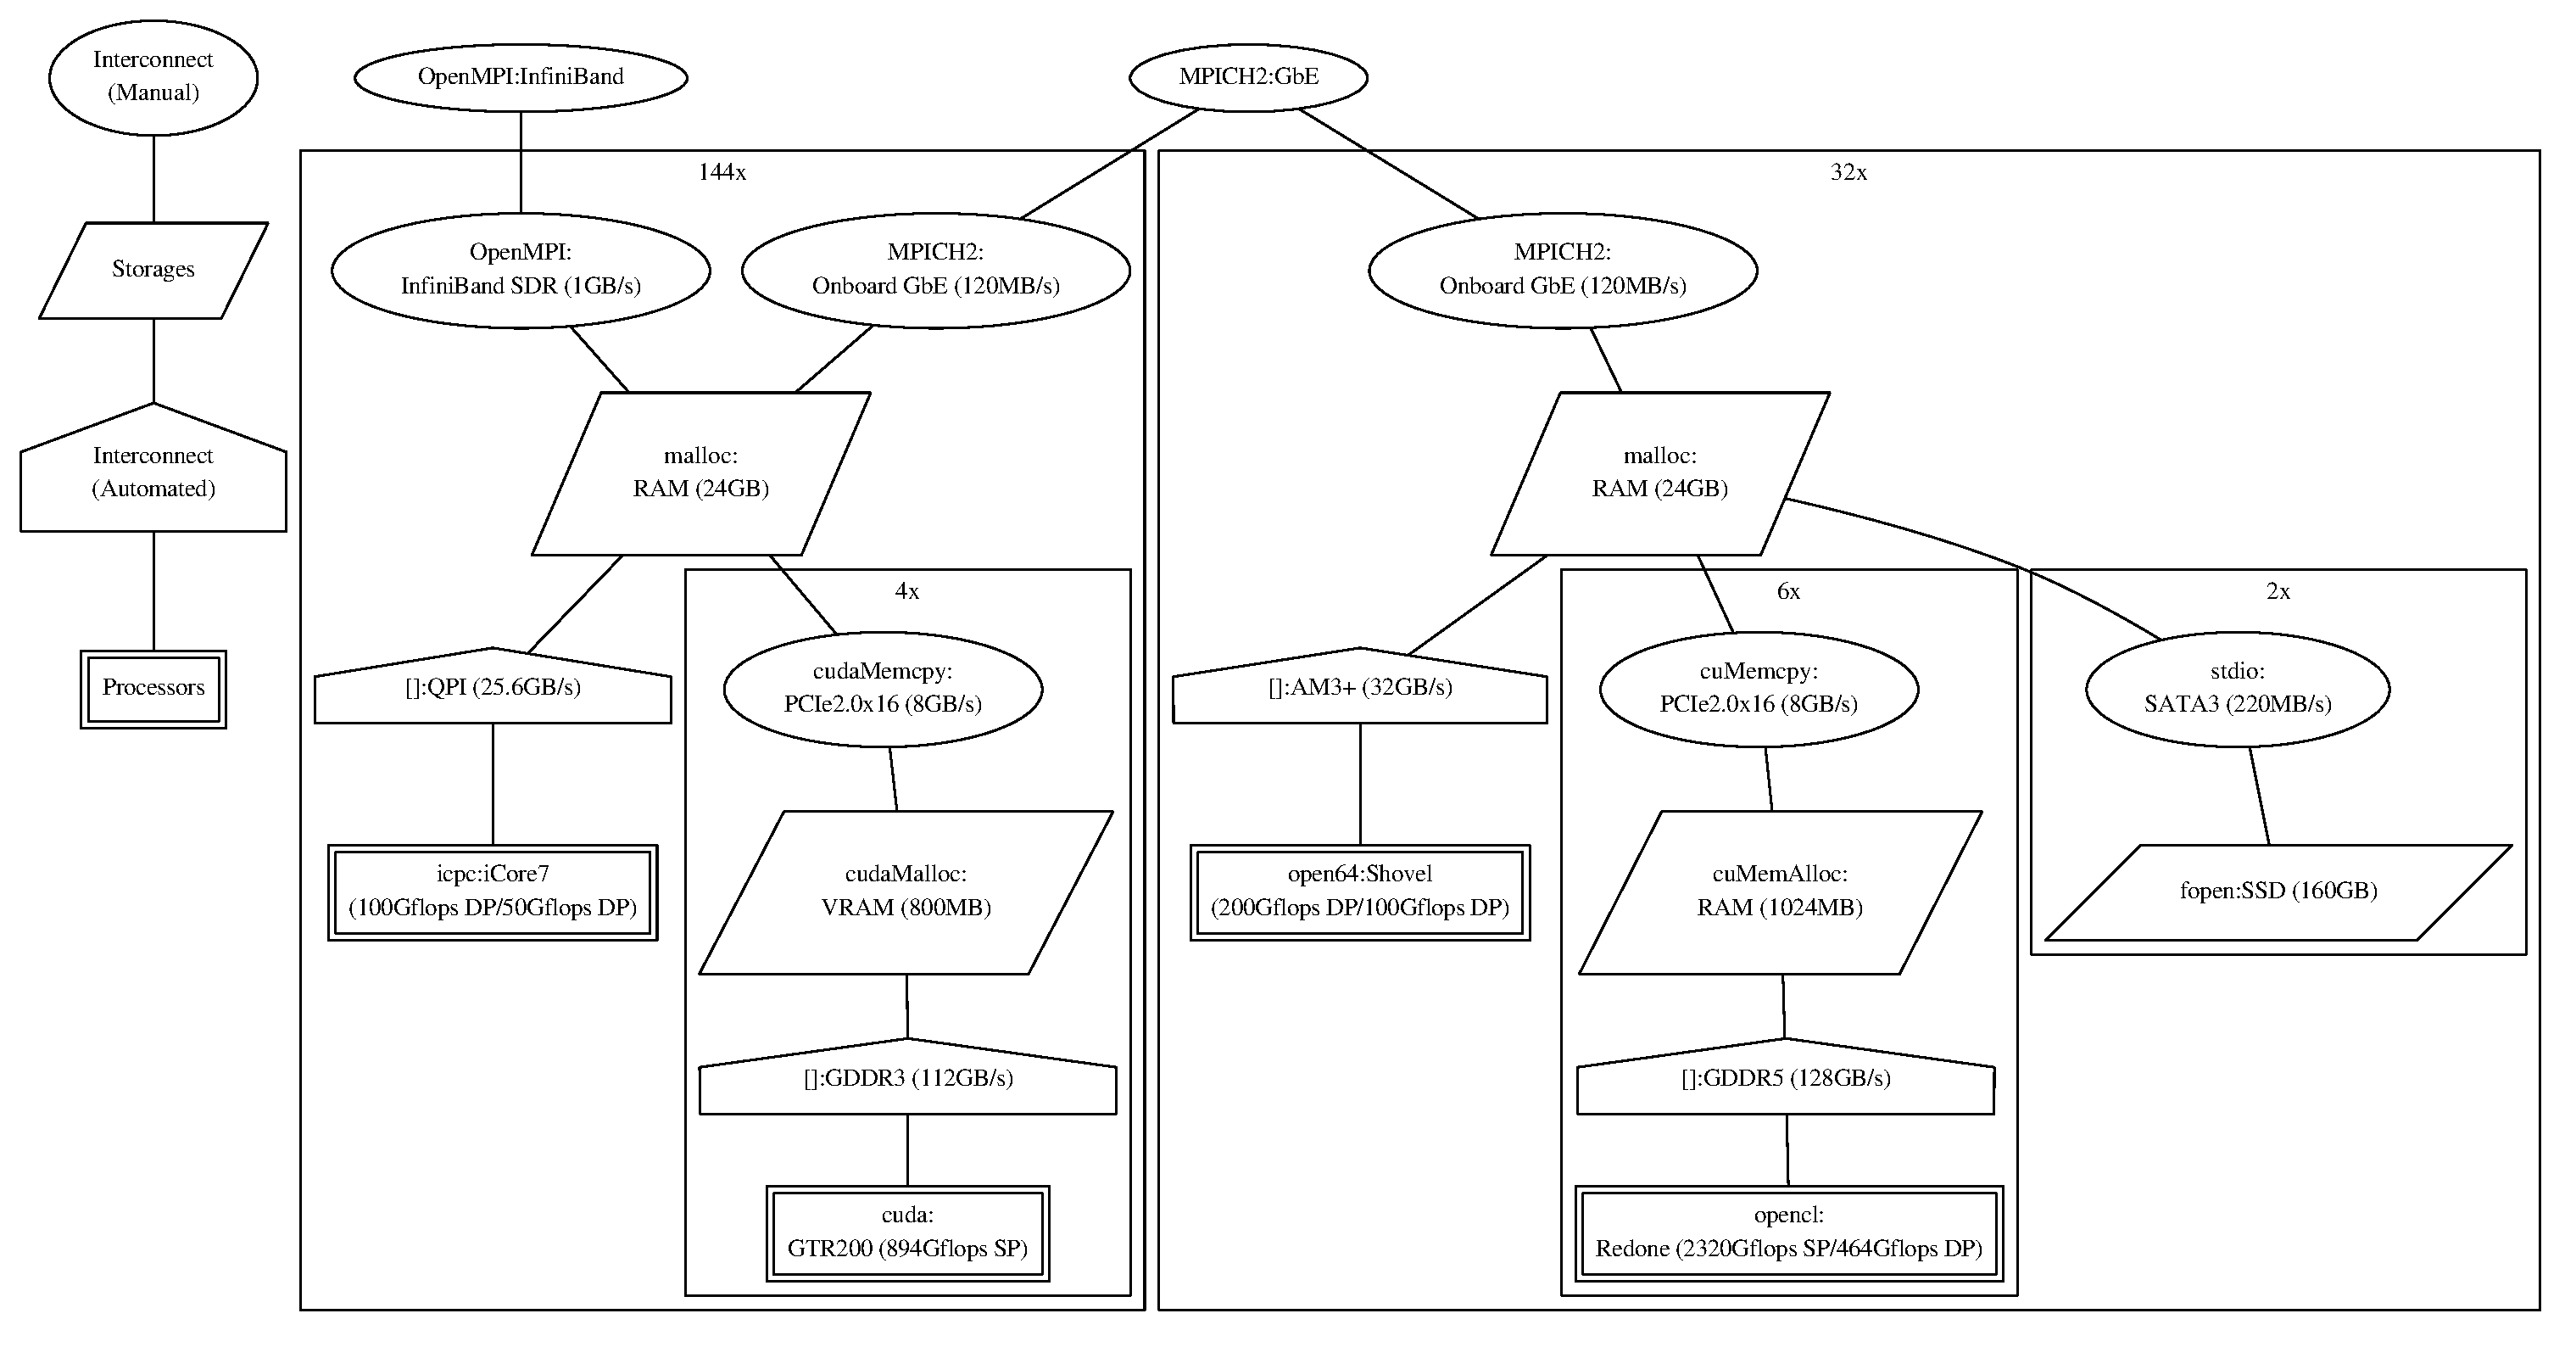
\includegraphics[scale=0.3]{figure/hardware_graph.eps}
  \end{center}
  \caption{Hardware model, generated from graphVis.}\label{FigureHardware}
\end{figure*}

\section{Instruction Set}

Orthotope Machine (OM) is a virtual machine that has an instruction set
operating on orthotopes. Each instruction is presented in static single
assignment (SSA) form. For example, {\tt add} instruction in common CPUs or in
LLVM adds two scalar value. The {\tt add} instruction in Orthotope Machine
takes two orthotope and returns one, acting much like {\tt zipWith (+)}.

\subsection{Static Addressed Single Assignment}

We extend the static single assignment (SSA) form concept to static addressed
single assignment(SASA) form.  Consider the following DPDEL program, where
{\tt a,b,c} are orthotopes:
\begin{verbatim}
b <- shift (-1) a * shift 1 a;
c <- shift (-1) b + b + shift (+1) b;
\end{verbatim}
the program is in SSA (static single assignment) form.
If we generate the following code from the DPDEL, it will give a wrong result.
\begin{verbatim}
double a[N], b[N], c[N];
for (int i=2; i<N-2; ++i) {
  b[i] =a[i-1]*a[i+1];
  c[i] =b[i-1]+b[i]+b[i+1];
}
\end{verbatim}
In parallel language such as CUDA, the execution order of the loop is
nondeterministic, so the result of the above program is not even
well-defined. In SSA (static single assignment) form, every variable is only
assigned once. However, there remains some ambiguity.  Assigning {\em each
  orthotope} variable only once does not fix the meaning of program uniquely
in such nondeterministically parallel environment.

One way to fix this is to assure that {\em each element of each orthotope} is
statically assigned at most once. To do this, first we must detect how the
output ({\tt c[i]} in this case) depends on every SSA orthotope and how large
is the stencil (dependency size). Then we can generate code like this:
\begin{verbatim}
double a[N], c[N];
for (int i=2; i<N-2; ++i) {
  a_i_minus_2 = a[i-2];
  a_i_minus_1 = a[i-1];
  a_i = a[i];
  a_i_plus_1 = a[i+1];
  a_i_plus_2 = a[i+2];
  b_i_minus_1 = a_i_minus_2 + a_i;
  b_i = a_i_minus_1 + a_i_plus_1;
  b_i_plus_1 = a_i + a_i_plus_2;
  c_i = b_i_minus_1 + b_i + b_i_plus_1;
  c[i] = c_i;
}
\end{verbatim}
Let us call this SASA (Static and Addressed Single Assignment)
form. Generating programs in SASA form introduces a lot of redundant
calculations. But it produces correct results.

At any point of time of execution, we can insert a global
synchronization, thus dividing the abstract syntax tree into several
parts, like this:

\begin{verbatim}
b <- shift (-1) a * shift 1 a;
-- cut here --
c <- shift (-1) b + b + shift (+1) b;
\end{verbatim}

From this AST, following code is generated:

\begin{verbatim}
double a[N], b[N], c[N];
for (int i=1; i<N-1; ++i) {
  a_i_minus_1 = a[i-1];
  a_i_plus_1 = a[i+1];
  b[i] = a_i_minus_1 + a_i_plus_1;
}
for (int i=2; i<N-2; ++i) {
  b_i_minus_1 = b[i-1];
  b_i = b[i];
  b_i_plus_1 = b[i+1];
  c_i = b_i_minus_1 + b_i + b_i_plus_1;
  c[i] = c_i;
}
\end{verbatim}

Synchronization insertion reduces the number of arithmetic operations
performed per mesh, at the cost of increased number of load/store
operations and increased storage consumption. Since the ratio of
calculation speed to storage access speed vary from hardware to
hardware, we need to search for the best number and place to insert
synchronizations for each hardware to achieve maximum performance .




\subsection{Instruction Set for Primordial Orthotope Machine}
Primordial OM is an imaginary machine with infinite amount of memory and
infinitely long vector arithmetric instructions. 
\subsection{Instruction Set for Distributed Orthotope Machine}

\section{Possible Program Transformations}
\subsection{Common Techniques}
A lot of important optimization techniques are known for scalar
processors. Some of them are equally applicable to Orthotope Machine
AST.  Even if we emit the code without such optimizations, we can
expect the native compilers do the job for us. At least Paraiso should
not hinder native optimizations. It's better if we can optimize OM AST
using modern optimization platform such as LLVM.

\paragraph{Constant Folding}
Constant folding is to calculate constant expression in compile
time. It'll be fairly easy, and if we forget to do it, native
compilers are also good at it. One very stupid thing is to store a
globally constant value onto an array. We should avoid this.

\paragraph{Loop Fusion}

Loop fusion is a source of high performance in Haskell's array operating
libraries {\tt Data.Vector} and {\tt Data.Array.Repa}, and also in many other
libraries in other languages.


\paragraph{Common Subexpression Elimination}

To avoid performing the same calculation twice, by storing the intermediate
value to the memory. 

\subsection{Time-step Fusion}
\subsection{Cache}
\subsection{Data-Flow-Tree Manipulations by User Specification}
\subsection{Synchronization Insertion}
\subsection{Trapezium Splitting}
\subsection{Parallelogram Splitting}
\subsection{Block Skew}
Fluid consists of multiple orthotope of the same shape and extent.
\subsection{Batch Reduce/Broadcast}
Reduce and broadcast needs global communications. To have large-grained
communications, it will be a good idea to perform many reduce/broadcast
instructions at once. 

It's good if we can detect the portions of calculations that do not depend on
the broadcast data, and perform such calculations in parallel while the
communications are going on.

\bibliography{paraiso}
\end{document}

